% Generative Forgery of Crowdsensed Sensor Streams: A Preliminary Evaluation of Trust Defenses -- IEEE PerCom 2027 Work-in-Progress results draft
% All reported results are generated from outputs_india_aqi/ with FAST=false and 3 seeds.
\documentclass[conference]{IEEEtran}
\usepackage{cite,amsmath,graphicx,booktabs,xcolor,url,microtype}
\begin{document}
\title{Generative Forgery of Crowdsensed Sensor Streams: A Preliminary Evaluation of Trust Defenses}
\author{\IEEEauthorblockN{Deepak Kambala}
\IEEEauthorblockA{Prism Labs\\University College of Engineering Narasaraopet (JNTUK), India\\deepakkambala@prism-labs.tech}}
\maketitle
\begin{abstract}
Crowdsensing defenses often rely on outlier filtering, truth discovery, or participant reputation. We evaluate these approaches against five forged stream types, including VAE and adaptive generators, using hourly Delhi air-quality stations. The conventional defenses have low true-positive rates at 5\% false positives against the learned forgers, and their aggregate error exceeds the undefended mean in this setup. A nine-feature gradient-boosted detector trained on white, replay, and AR forgeries reaches AUROC 0.991 $\pm$ 0.002 on unseen VAE streams and 0.963 $\pm$ 0.005 on adaptive streams. Its feature ablation and attacker-proxy sweeps reveal a less simple result than expected: intrinsic features alone match the full detector on these attacks, while coupled-only features are weaker; adaptive AUROC also declines as proxy smoothing grows. Feature extraction takes 1.15,ms per stream in the notebook's single-core timing.
\end{abstract}
\begin{IEEEkeywords}
mobile crowdsensing, Sybil attack, generative forgery, truth discovery, anomaly detection
\end{IEEEkeywords}
\section{Introduction}
Mobile crowdsensing lets phones and low-cost sensors contribute measurements such as air quality, noise, and traffic~\cite{ganti2011}. Open participation invites Sybil attacks, in which one adversary controls many fake identities~\cite{douceur2002}. Common defenses filter outliers, estimate source reliability through truth discovery~\cite{li2014crh,li2016survey}, or weight participants by reputation. These methods can struggle when forged data reproduces realistic temporal patterns.

We study generated sensor-stream forgeries anchored to a public proxy of the honest consensus, with a bias on selected channels. We compare three conventional defenses, a supervised detector trained only on crude forgeries, and a label-free Isolation Forest. Our goal is to measure their relative behavior on a single real-world station dataset, not to claim independent ground truth or universal robustness.
\section{Threat Model and Forgers}
A campaign has $N_h$ honest participants and Sybils reporting $R$ consecutive windows of $L$ hourly samples over $C$ channels. The attacker biases PM$_{2.5}$ and PM$_{10}$ by $\delta$ standard deviations. Its forged stream is a smoothed public proxy of the honest median plus the shift and a generated deviation. Proxy smoothing $k{=}1$ is the real-time setting; larger $k$ uses a more smoothed reference. Forgers are white noise, replayed deviations, fitted AR(1), an MLP-VAE, and an adaptive best-of-$K$ VAE sample chosen for intrinsic-feature similarity ($K{=}50$). Generators use the first 60\% of the timeline; evaluation uses the last 40\%.
\section{Detector}
For each stream we form the residual from a leave-one-out median and compute nine features. Six intrinsic features summarize lag-1 autocorrelation, spectral flatness, high-frequency power, kurtosis, cross-channel correlation, and heteroscedasticity. Three consensus-coupled features measure first-difference correlation, residual RMSE, and absolute bias. Gradient-boosted models use all features or either feature group; training includes white, replay, and AR attacks only. The label-free variant fits an Isolation Forest to honest streams and sets its threshold at the 95th percentile of honest scores. Flagged streams are removed before aggregation.
\section{Experimental Setup}
We use the Kaggle Air Quality Data in India hourly records~\cite{rao2020aqi}: 30 Delhi stations with usable coverage over Jan. 2018--Jun. 2020, and PM$_{2.5}$, PM$_{10}$, NO$_2$, CO, and SO$_2$. Values are log-transformed and standardized; no honest sensor noise is simulated. The setup uses $L{=}48$, $R{=}4$, $N_h{=}20$, Sybil fraction $\rho{=}0.3$, shift $\delta{=}0.4$, proxy noise $0.05$, 150 training and 100 test campaigns per forger, and three seeds. Metrics are stream AUROC, TPR at 5\% FPR, and aggregate error on attacked channels (standardized units). The campaign honest mean is the reference; the dataset provides no independent truth for this experiment.
The station traces share temporal structure but retain substantial station-specific variation.
\begin{figure}[t]
\centering
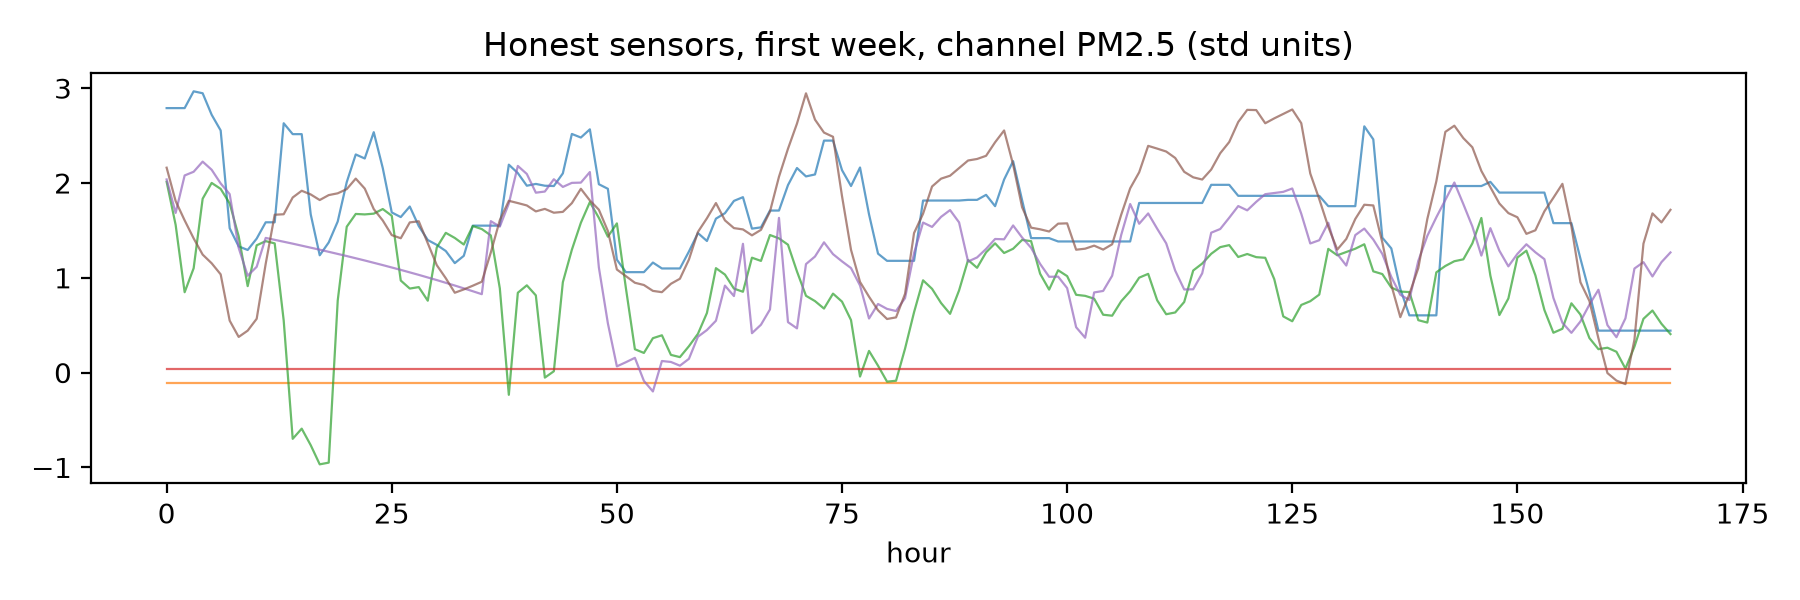
\includegraphics[width=\columnwidth]{outputs_india_aqi/fig0_honest.png}
\caption{Honest Delhi station streams during the first week.}
\label{fig:honest}
\end{figure}
\section{Results}
\textbf{Conventional defenses underperform against learned streams.} For VAE/adaptive attacks, their AUROCs range from 0.609 $\pm$ 0.006 (truth discovery, VAE) to 0.772 $\pm$ 0.001 (MAD, adaptive), while TPR@5\%FPR ranges from 0.001 $\pm$ 0.000 to 0.105 $\pm$ 0.007. TPR and aggregate-error results are listed in Tables~\ref{tab:tpr} and~\ref{tab:aggerr}. On VAE/adaptive attacks, undefended aggregate error is 0.137 $\pm$ 0.002/0.118 $\pm$ 0.008; MAD gives 0.255 $\pm$ 0.008/0.237 $\pm$ 0.008, truth discovery 0.183 $\pm$ 0.005/0.147 $\pm$ 0.008, and reputation 0.151 $\pm$ 0.003/0.126 $\pm$ 0.008. Thus all three increase error relative to the undefended mean in these two settings.

\textbf{Detector and ablation.} Full GBM obtains VAE/adaptive AUROC 0.991 $\pm$ 0.002/0.963 $\pm$ 0.005 and TPR@5\%FPR 0.951 $\pm$ 0.015/0.768 $\pm$ 0.033. Intrinsic-only is 0.990 $\pm$ 0.001/0.964 $\pm$ 0.008, essentially tied with the full feature set on these attacks. Coupled-only is lower at 0.811 $\pm$ 0.009/0.757 $\pm$ 0.023. The measured ablation therefore does not support the expectation that coupled features alone carry the defense. Isolation Forest reaches AUROC 0.987 $\pm$ 0.002/0.913 $\pm$ 0.009 and TPR 0.964 $\pm$ 0.007/0.506 $\pm$ 0.049; it is weak on replay (AUROC 0.537 $\pm$ 0.018, TPR 0.100 $\pm$ 0.015) and AR (AUROC 0.634 $\pm$ 0.018, TPR 0.089 $\pm$ 0.007).

\textbf{Sweeps and observed anomaly.} As Sybil fraction rises from 0.1 to 0.5, full-GBM VAE aggregate error increases from 0.018 to 0.040; MAD increases from 0.181 to 0.323. As shift rises from 0.1 to 0.8, full-GBM AUROC remains 0.991--0.993 and its error changes from 0.025 to 0.031, while baseline errors rise. In the adaptive proxy sweep, full-GBM AUROC falls from 0.964 at $k{=}1$ to 0.677 at $k{=}24$ (TPR from 0.807 to 0.099); intrinsic-only falls from 0.967 to 0.863. This direction is opposite the notebook's expected easier-detection trend for increasingly smoothed, weaker attacker proxies. The result is reported as observed and merits follow-up.

\textbf{Cost.} The recorded feature extraction time is 1.15 ms per stream in the notebook's single-core timing; it is a microbenchmark, not an end-to-end deployment measurement.
\begin{figure}[t]
\centering
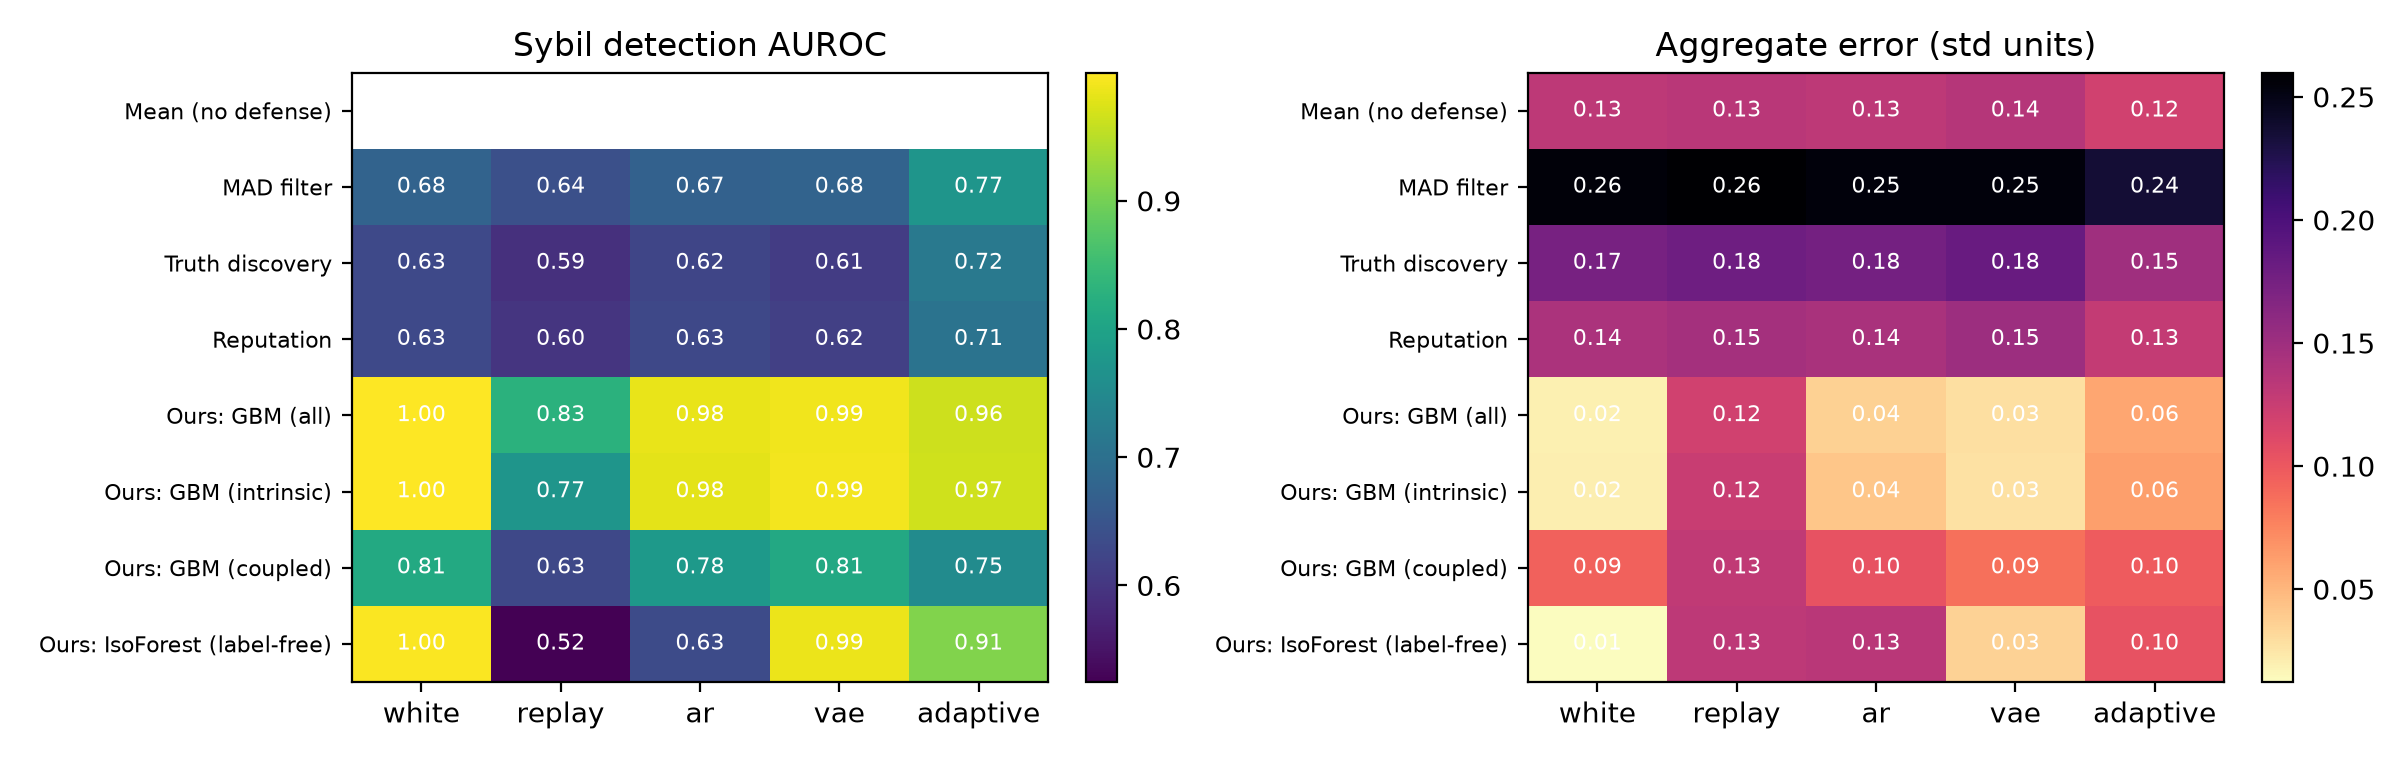
\includegraphics[width=\columnwidth]{outputs_india_aqi/fig1_main_heatmaps.png}
\caption{Mean AUROC and aggregate error for each defense and forger.}
\label{fig:heat}
\end{figure}
\begin{table}[t]
\centering
\caption{AUROC, mean $\pm$ standard deviation over three seeds.}
\label{tab:auroc}
\resizebox{\columnwidth}{!}{\begin{tabular}{llllll}
\toprule
forger & white & replay & ar & vae & adaptive \\
method &  &  &  &  &  \\
\midrule
Mean (no defense) & -- & -- & -- & -- & -- \\
MAD filter & 0.68 $\pm$ 0.01 & 0.64 $\pm$ 0.01 & 0.67 $\pm$ 0.01 & 0.68 $\pm$ 0.01 & 0.77 $\pm$ 0.01 \\
Truth discovery & 0.63 $\pm$ 0.01 & 0.59 $\pm$ 0.0 & 0.62 $\pm$ 0.0 & 0.61 $\pm$ 0.01 & 0.72 $\pm$ 0.01 \\
Reputation & 0.63 $\pm$ 0.0 & 0.6 $\pm$ 0.0 & 0.63 $\pm$ 0.0 & 0.62 $\pm$ 0.01 & 0.71 $\pm$ 0.01 \\
Ours: GBM (all) & \textbf{1.0 $\pm$ 0.0} & \textbf{0.83 $\pm$ 0.0} & \textbf{0.98 $\pm$ 0.0} & 0.99 $\pm$ 0.0 & 0.96 $\pm$ 0.01 \\
Ours: GBM (intrinsic) & 1.0 $\pm$ 0.0 & 0.77 $\pm$ 0.0 & 0.98 $\pm$ 0.0 & \textbf{0.99 $\pm$ 0.0} & \textbf{0.97 $\pm$ 0.01} \\
Ours: GBM (coupled) & 0.81 $\pm$ 0.0 & 0.63 $\pm$ 0.01 & 0.78 $\pm$ 0.01 & 0.81 $\pm$ 0.01 & 0.75 $\pm$ 0.02 \\
Ours: IsoForest (label-free) & 1.0 $\pm$ 0.0 & 0.52 $\pm$ 0.02 & 0.63 $\pm$ 0.03 & 0.99 $\pm$ 0.0 & 0.91 $\pm$ 0.01 \\
\bottomrule
\end{tabular}
}
\end{table}
\begin{table*}[!t]
\centering
\scriptsize
\caption{TPR at 5\% FPR, mean $\pm$ standard deviation over three seeds.}
\label{tab:tpr}
\resizebox{0.82\textwidth}{!}{\begin{tabular}{llllll}
\toprule
forger & white & replay & ar & vae & adaptive \\
method &  &  &  &  &  \\
\midrule
Mean (no defense) & -- & -- & -- & -- & -- \\
MAD filter & 0.07 $\pm$ 0.01 & 0.07 $\pm$ 0.01 & 0.07 $\pm$ 0.01 & 0.03 $\pm$ 0.01 & 0.1 $\pm$ 0.01 \\
Truth discovery & 0.04 $\pm$ 0.01 & 0.03 $\pm$ 0.0 & 0.03 $\pm$ 0.0 & 0.01 $\pm$ 0.0 & 0.02 $\pm$ 0.01 \\
Reputation & 0.01 $\pm$ 0.0 & 0.01 $\pm$ 0.0 & 0.01 $\pm$ 0.0 & 0.0 $\pm$ 0.0 & 0.01 $\pm$ 0.0 \\
Ours: GBM (all) & \textbf{1.0 $\pm$ 0.0} & \textbf{0.33 $\pm$ 0.01} & \textbf{0.92 $\pm$ 0.0} & 0.95 $\pm$ 0.02 & 0.8 $\pm$ 0.05 \\
Ours: GBM (intrinsic) & 1.0 $\pm$ 0.0 & 0.24 $\pm$ 0.01 & 0.91 $\pm$ 0.01 & \textbf{0.96 $\pm$ 0.0} & \textbf{0.83 $\pm$ 0.07} \\
Ours: GBM (coupled) & 0.18 $\pm$ 0.02 & 0.12 $\pm$ 0.01 & 0.17 $\pm$ 0.01 & 0.21 $\pm$ 0.02 & 0.14 $\pm$ 0.03 \\
Ours: IsoForest (label-free) & 1.0 $\pm$ 0.0 & 0.1 $\pm$ 0.01 & 0.08 $\pm$ 0.02 & 0.96 $\pm$ 0.0 & 0.49 $\pm$ 0.02 \\
\bottomrule
\end{tabular}
}
\end{table*}
\begin{table*}[!t]
\centering
\scriptsize
\caption{Aggregate error on attacked channels (standardized units), mean $\pm$ standard deviation.}
\label{tab:aggerr}
\resizebox{0.82\textwidth}{!}{\begin{tabular}{llllll}
\toprule
forger & white & replay & ar & vae & adaptive \\
method &  &  &  &  &  \\
\midrule
Mean (no defense) & 0.13 $\pm$ 0.0 & 0.13 $\pm$ 0.0 & 0.13 $\pm$ 0.0 & 0.14 $\pm$ 0.0 & 0.12 $\pm$ 0.01 \\
MAD filter & 0.26 $\pm$ 0.01 & 0.26 $\pm$ 0.01 & 0.25 $\pm$ 0.01 & 0.25 $\pm$ 0.01 & 0.24 $\pm$ 0.01 \\
Truth discovery & 0.17 $\pm$ 0.01 & 0.18 $\pm$ 0.01 & 0.18 $\pm$ 0.0 & 0.18 $\pm$ 0.01 & 0.15 $\pm$ 0.01 \\
Reputation & 0.14 $\pm$ 0.0 & 0.15 $\pm$ 0.0 & 0.14 $\pm$ 0.0 & 0.15 $\pm$ 0.0 & 0.13 $\pm$ 0.01 \\
Ours: GBM (all) & 0.02 $\pm$ 0.0 & \textbf{0.12 $\pm$ 0.0} & \textbf{0.04 $\pm$ 0.0} & 0.03 $\pm$ 0.01 & \textbf{0.06 $\pm$ 0.01} \\
Ours: GBM (intrinsic) & 0.02 $\pm$ 0.0 & 0.12 $\pm$ 0.0 & 0.04 $\pm$ 0.0 & \textbf{0.03 $\pm$ 0.0} & 0.06 $\pm$ 0.01 \\
Ours: GBM (coupled) & 0.09 $\pm$ 0.0 & 0.13 $\pm$ 0.0 & 0.1 $\pm$ 0.01 & 0.09 $\pm$ 0.0 & 0.1 $\pm$ 0.0 \\
Ours: IsoForest (label-free) & \textbf{0.01 $\pm$ 0.0} & 0.13 $\pm$ 0.0 & 0.13 $\pm$ 0.0 & 0.03 $\pm$ 0.0 & 0.1 $\pm$ 0.01 \\
\bottomrule
\end{tabular}
}
\end{table*}
\begin{figure*}[t]
\centering
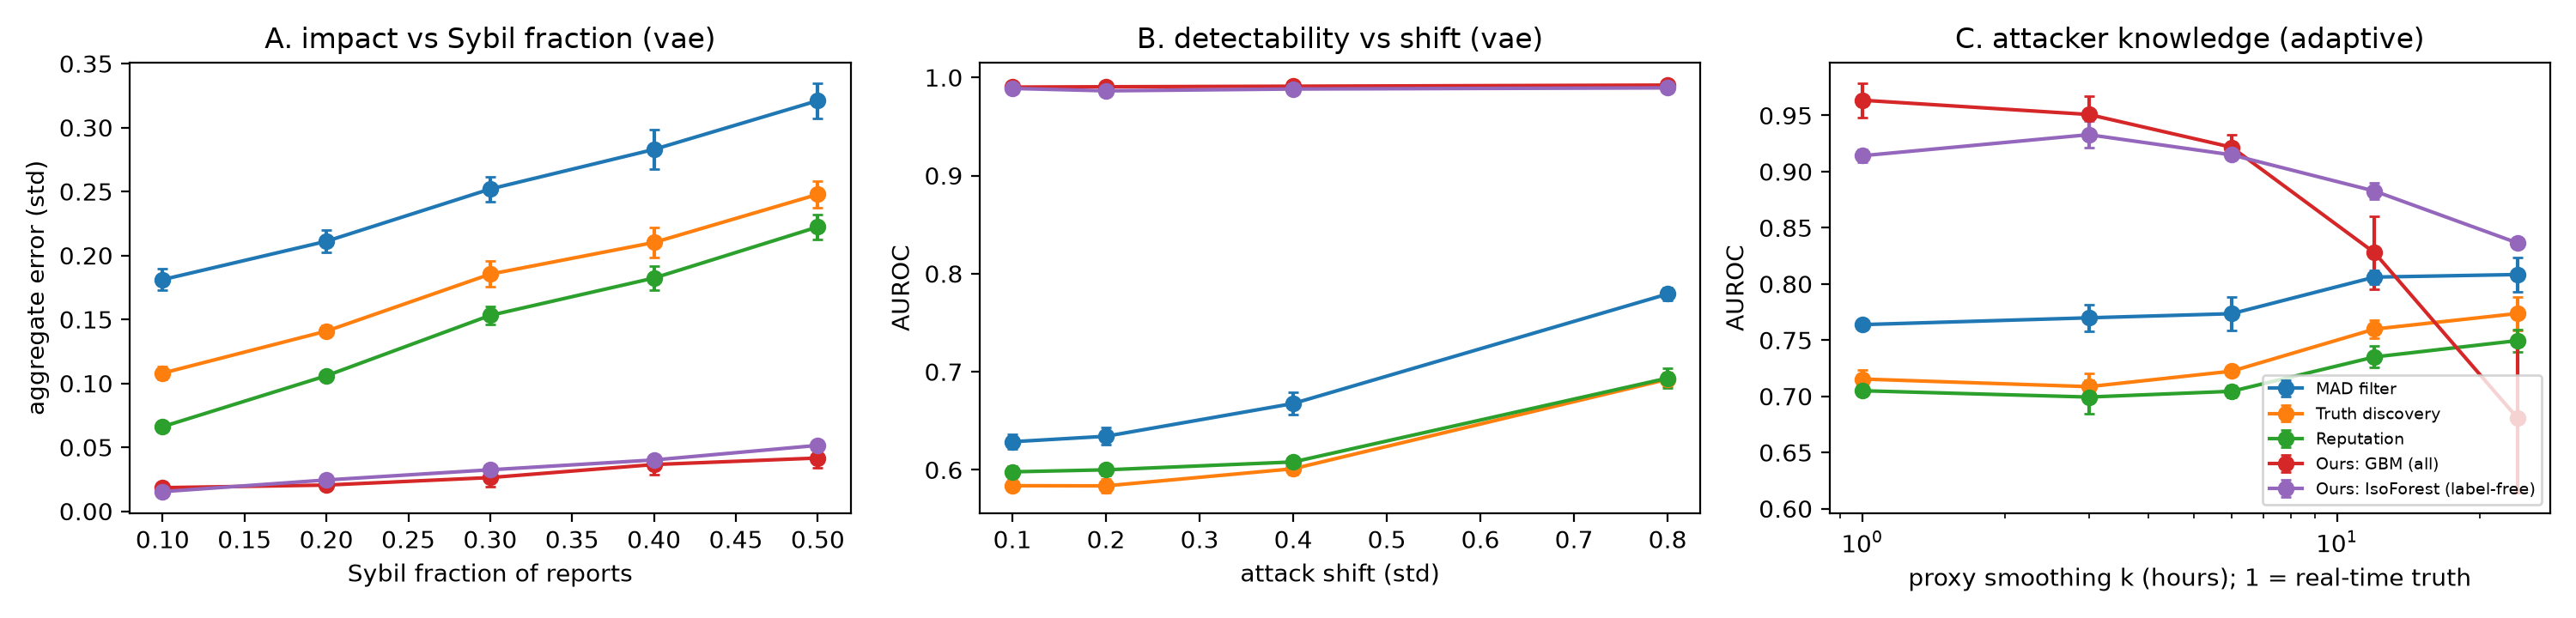
\includegraphics[width=0.95\textwidth]{outputs_india_aqi/fig4_sweeps.png}
\caption{A: aggregate error versus Sybil fraction. B: VAE detectability versus shift. C: adaptive detectability versus proxy smoothing $k$.}
\label{fig:sweeps}
\end{figure*}
\textbf{Discussion.} The no-defense aggregate error is already modest, so the main practical effect here is whether screening removes Sybils without rejecting too many honest participants. The strict 5\% FPR results expose a gap hidden by AUROC, especially for the label-free model on adaptive streams and for every baseline. The high VAE scores for both GBM feature settings show generalization beyond the three training forgers in this data split, while the poor replay result for Isolation Forest cautions against treating a one-class model as a universal fallback. The proxy-resolution sweep is particularly important: its direction contradicts the expected relation between stale attacker knowledge and detectability. The proxy is regenerated and the VAE is retrained at each $k$, so this curve should be rechecked before making a causal claim about proxy freshness.

The qualitative and feature-importance plots provide context for these aggregate metrics, but the paper does not treat visual similarity or feature importance as independent evidence of robustness.
\begin{figure*}[!t]
\centering
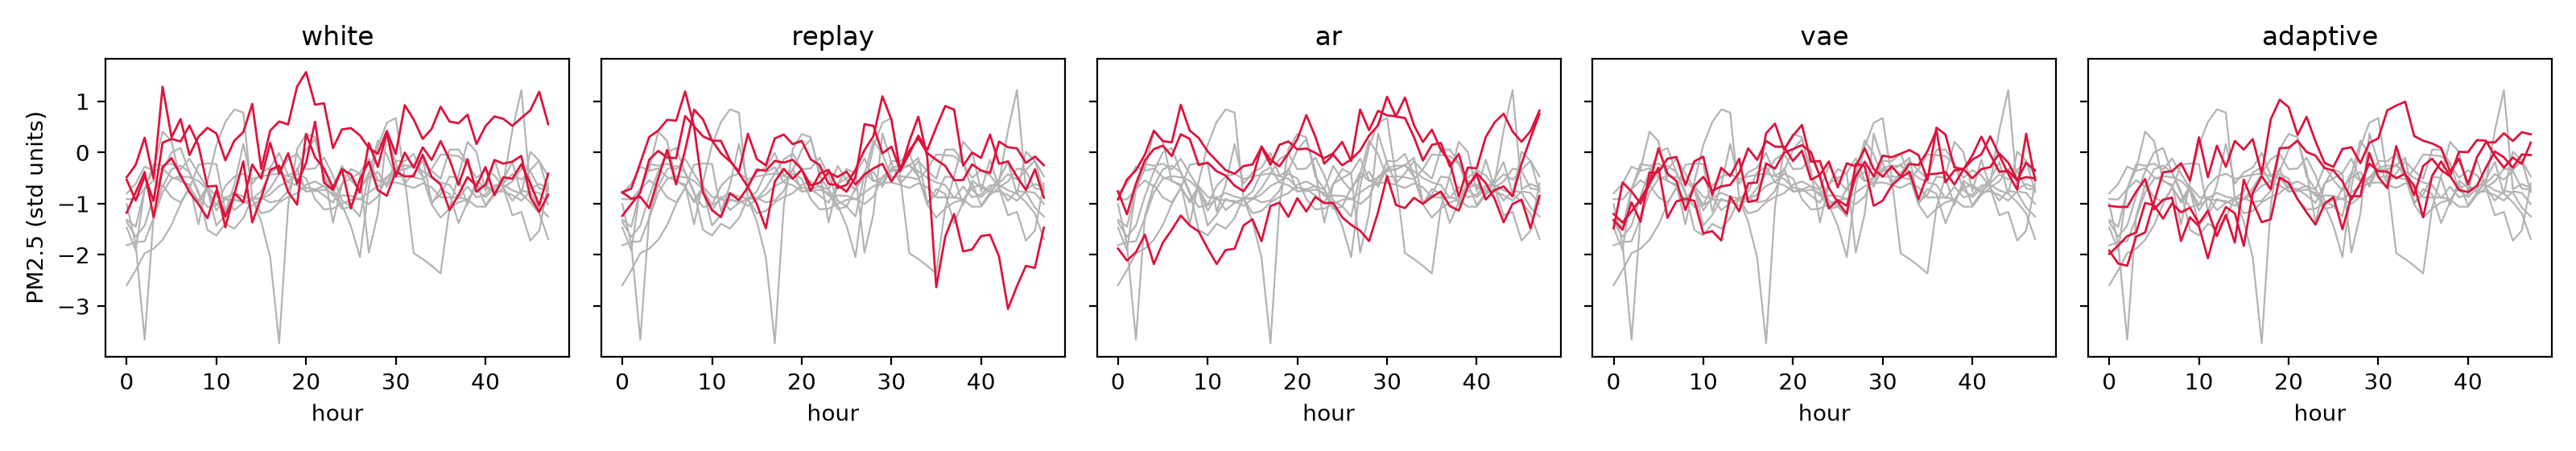
\includegraphics[width=0.95\textwidth]{outputs_india_aqi/fig3_forged_vs_honest.png}
\caption{Example honest and forged PM$_{2.5}$ streams from one test window.}
\label{fig:streams}
\end{figure*}
Feature importance is concentrated in cross-channel residual correlation, with kurtosis and high-frequency power next in the exported ranking (Fig.~\ref{fig:importance}). This description is consistent with the intrinsic-only ablation, but it does not establish which individual feature causes detection.
\begin{figure*}[!t]
\centering
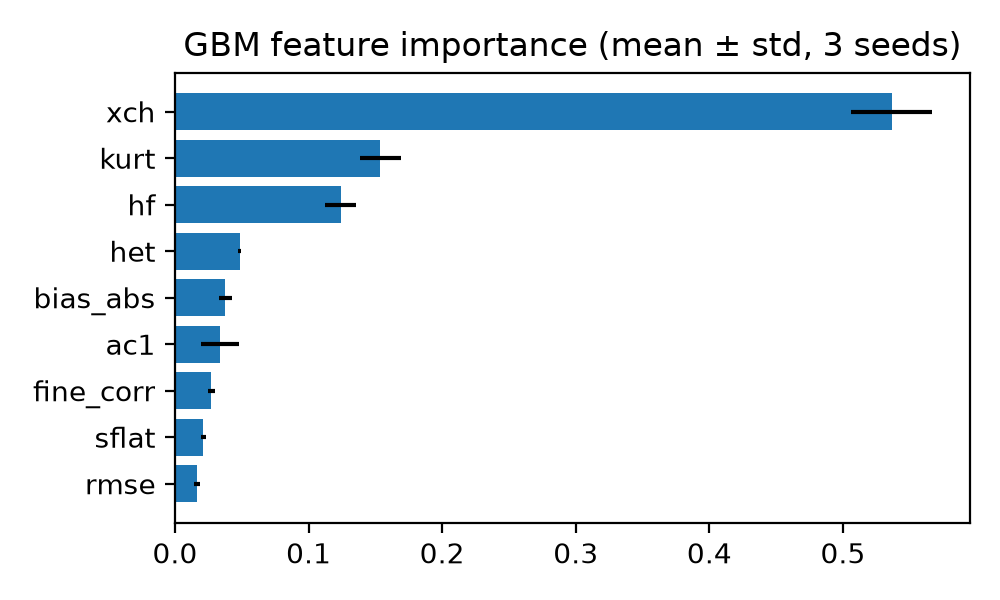
\includegraphics[width=0.98\textwidth]{outputs_india_aqi/fig2_feature_importance.png}
\caption{GBM feature importance across three seeds.}
\label{fig:importance}
\end{figure*}
\section{Limitations and Conclusion}
These experiments use one city and the honest-sensor consensus as a reference, not independent ground truth. The adaptive generator optimizes intrinsic statistics only; multi-city data, attacks tuned to the full detector, and deployment measurements remain future work. Under this protocol, conventional defenses increase aggregate error against the learned attacks. The full GBM detects them well, but the feature ablation and proxy sweep expose results that differ from the initial hypothesis and should be validated independently.
\begin{thebibliography}{99}
\bibitem{ganti2011} R. K. Ganti, F. Ye, and H. Lei, ``Mobile crowdsensing: current state and future challenges,'' \emph{IEEE Commun. Mag.}, vol. 49, no. 11, 2011.
\bibitem{douceur2002} J. R. Douceur, ``The Sybil attack,'' in \emph{Proc. IPTPS}, 2002.
\bibitem{li2014crh} Q. Li \emph{et al.}, ``Resolving conflicts in heterogeneous data by truth discovery and source reliability estimation,'' in \emph{Proc. ACM SIGMOD}, 2014.
\bibitem{li2016survey} Y. Li \emph{et al.}, ``A survey on truth discovery,'' \emph{ACM SIGKDD Explorations}, vol. 17, no. 2, 2016.
\bibitem{friedman2001} J. H. Friedman, ``Greedy function approximation: a gradient boosting machine,'' \emph{Ann. Statist.}, vol. 29, no. 5, 2001.
\bibitem{liu2008} F. T. Liu, K. M. Ting, and Z.-H. Zhou, ``Isolation forest,'' in \emph{Proc. IEEE ICDM}, 2008.
\bibitem{rao2020aqi} R. Rao, ``Air quality data in India (2015--2020),'' Kaggle dataset.
\end{thebibliography}
\end{document}
